\documentclass{article}
\usepackage{ctex}
\usepackage{amsmath}
\usepackage{graphicx}
\usepackage{tikz}

\title{数据结构第一次作业}
\author{陈小羽}
\date{}

\begin{document}
\maketitle
\tableofcontents
\section{题目要求}
	\paragraph{}
		\begin{itemize}
			\item 创建电话号码本可以存储每个人的(姓名,地址,电话号码),一个人可以有多个电话号码,但所有电话号码不能有重复;
			\item 可以根据电话号码对人的信息进行排序;
			\item 可以根据姓名查询这个人的所有电话号码和地址;如果查询失败,则询问是否添加这个人的信息到电话号码本中,
			如果``Yes'',则根据输入的姓名,电话号码,地址等信息添加到电话号码本程序中;
			\item 可以根据电话号码查询对应的人的信息:姓名和地址,并删除或修改该人的信息;
			\item 要求查询和排序速度尽量快
		\end{itemize}
\section{数据结构的选择}
	\paragraph{}
		根据题目的要求,我们需要做到快速地访问,插入,查询元素。还要能够将数据按照键值排序。
		按照题目中速度越快越好的要求,我选择了著名计算机科学家Tarjan于1985年提出的\textbf{伸展树}结构。
\subsection{基本操作}
	\paragraph{}
		根据我们的储备知识,再结合题目中的要求,我们需要实现\textbf{伸展树}的如下操作。
		\begin{itemize}
			\item access\_L(key): 找到并返回第一个键值不大于key的结点的位置。并将这个结点旋转到根节点。
			\item access\_R(key): 找到并返回第一个键值大于key的结点的位置。并将这个结点旋转到根节点。
			\item access(key): 返回键值为key的结点。
			\item splay(node): 将node结点旋转到根节点。在每次访问了一个结点之后使用。
			\item insert(key): 将一个键值为key的点加入树中。
			\item delete(key): 将树中键值为key的结点删除。
			\item query(key): 查询键值为key的结点中储存的信息。
			\item dfs(): 按照中序遍历访问整棵树,达到题目中对数据进行排序的要求。
		\end{itemize}
		下面我们来具体的描述和分析这些操作。
	\subsubsection{splay}
		\paragraph{}
			splay操作是整个数据结构的最重要的操作,也是整个算法的效率的保证。他的作用是将最近访问过的结点,
			和一些有特定需要的点,按照一定的方式旋转到根节点。splay操作可以保证算法的所有操作的均摊复杂度
			是$\mathcal{O}(logn)$的。
		\paragraph{旋转}
			在将一个结点移动到根节点的过程中,我们需要使用一种叫做旋转的操作来保证左右儿子的相对大小关系。
			和时间复杂度。对于伸展树,我们具体有3种旋转的方法。
			\begin{center}
			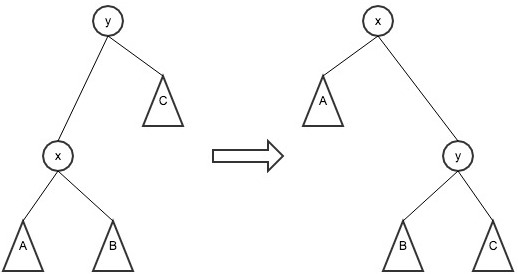
\includegraphics[width = 11cm]{zig.jpg}\\
			\end{center}
			zig: 将一个结点旋转到它的父亲结点的位置,然后让它的父亲结点变成它的一个儿子结点。
			\begin{center}
			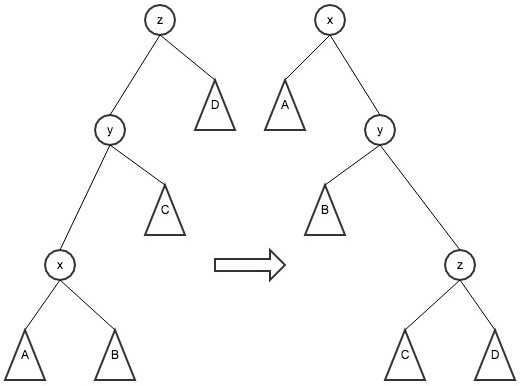
\includegraphics[width = 11cm]{zig-zig.jpg}\\
			\end{center}
			zig-zig: 如果一个点和它的父亲结点位于相同的子树(左/右)的时候,直观看起来是一条线,执行zig-zig.
			具体做法是,先对y做一次zig,然后对x做一次zig。
			\begin{center}
			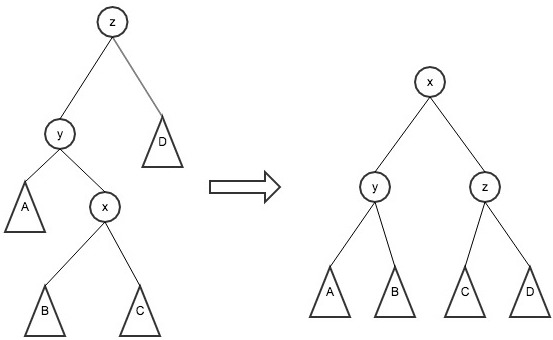
\includegraphics[width = 11cm]{zig-zag.jpg}\\
			\end{center}
			zig-zag: 如果一个点和它的父亲结点在不同的子树,那么执行zig-zag, 具体做法是对x进行2次zig操作。
		\paragraph{}
			显然,对一个结点连续使用三种旋转,就能将其旋转到根节点。
		\paragraph{代码}
			\begin{center}
			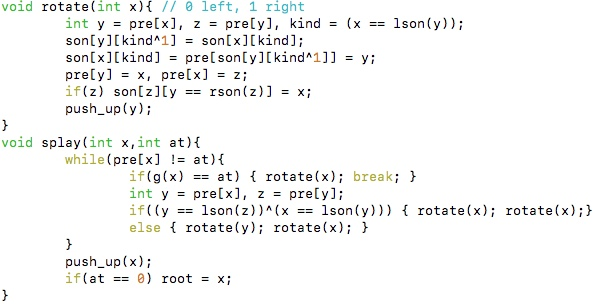
\includegraphics[width = 13cm]{splay_code.jpeg}\\
			\end{center}
	\subsubsection{access}
		\paragraph{}
			access函数的功能具体由access\_L和access\_R来提供,这两个函数的功能相当于在具体的序列上二分查找
			满足要求的结点。要实现函数的功能,我们需要维护每棵子树中的最小值和最大值。
		\paragraph{代码}
			\begin{center}
			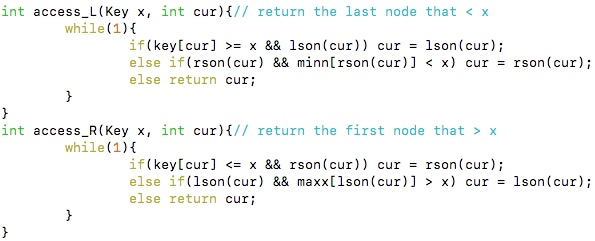
\includegraphics[width = 13cm]{access_code.jpeg}\\
			\end{center}
	\subsubsection{delete, insert, query, dfs}
		这些操作都可以用前面的操作拼凑出来。就显得没有那么的重要了。
\subsection{复杂度分析}
	这里我们主要想要说明,每一次splay操作的均摊复杂度为$\mathcal{O}(logn)$。由此很容易就能在同样的均摊复杂度下
	实现题目中要求的所有的操作(除了dfs输出排序结果是$\mathcal{O}(n)$的)。
	\subsubsection{势}
		\paragraph{}
			我们定义一种\textbf{势函数}来衡量当前图的状态,用来更好的分析时间复杂度。
			我们给每个结点一个权值$w(i)$.
			记图中以某个结点为根的子树的权值之和$S(x)$,则每个点的是函数定义为$\Phi (x) = \log S(x)$。
			定义整个树的势函数为$\Phi = \sum \Phi(x)$
	\subsubsection{摊还时间}
		\paragraph{}
			我们为每次操作的摊还时间$a = t + \Phi' - \Phi$。其中$t$是操作实际的时间,$\Phi'$是操作过后,整个
			树的势,$\Phi$是操作之前整棵树的势。
			然后我们就可以发现,对于连续的$m$次操作。总的时间可以表示为:
			\begin{displaymath}
				\sum_{j=1}^m t_j = \sum_{j=1}^m (a_j + \Phi_{j-1} - \Phi_j) = \sum_{j=1}^m a_j + \Phi_0 - \Phi_m
			\end{displaymath}
		\paragraph{}
			现在我们来分析每一次旋转操作的摊还时间。
			\begin{itemize}
				\item zig: \\
				$a = 1 + \Phi'(x) + \Phi'(y) - \Phi(x) - \Phi(y)$ 只有x和y的势会变化。 \\
				$\leq 1 + \Phi'(x) - \Phi(x)$, 因为$\Phi(y) \geq \Phi'(y)$ \\
				$\leq 1 + 3(\Phi'(x) - \Phi(x))$,因为$\Phi'(x) \geq \Phi(x)$ 
				\item zig-zig: \\
				$a = 2 + \Phi'(x) + \Phi'(y) + \Phi'(z) - \Phi(x) - \Phi(y) - \Phi(z)$, 只有x,y,z的势发生了变化。\\
				$= 2 + \Phi'(y) + \Phi'(z) - \Phi(x) - \Phi(y)$, 因为$\Phi'(x) = \Phi'(z)$ \\
				$\leq 2 + \Phi'(x) + \Phi'(z) - 2\Phi(x)$, 因为$\Phi'(x) \geq \Phi'(y)$且$\Phi(y) \geq \Phi(x)$\\
				又因为对于所有的$x+y \leq 1$且$x,y > 0$,都有$\max\{\log x + \log y\} = -2$,所以
				$\Phi(x) + \Phi'(z) - 2\Phi'(x) = \log(S(x)/S'(x)) + \log(S'(z)/S'(x)) \leq -2$
				将这个式子带上去就可以得到\\$\leq 3(\Phi'(x) - \Phi(x))$.
				\item zig-zag: \\
				$2 + \Phi'(x) + \Phi'(y) + \Phi'(z) - \Phi(x) - \Phi(y) - \Phi(z)$ \\
				$\leq 2 + \Phi'(y) + \Phi'(z) - 2\Phi(x)$, 因为$\Phi'(x) = \Phi(z)$ 且$\Phi(x) \leq \Phi(y)$\\
				和zig-zig使用同样的方法,最后可以得到\\
				$\leq 2(\Phi'(x) - \Phi(x)) \leq 3(\Phi'(x) - \Phi(x))$
			\end{itemize}
			综上所述,一次splay中产出的摊还时间的和应该为: $3(\Phi(t) - \Phi(x)) + 1$。(zig的情况多了一个一,但是
			我们在单次spaly操作中,最多只会用到一次zig。)
			而$3(\Phi(t) - \Phi(x)) + 1 = \mathcal{O}(log(S(t)/S(x)))$
		\paragraph{}
			设整棵树的势的大小为$W$, 显然$W = S(root)$现在假设我们已经做了$m$次splay操作。
			则$\sum_{j=1}^m a_j = m \times \mathcal{O}(log(S(t)/S(x)) = m \times \mathcal{O}(log(W/S(x)))$
			即:
			\begin{displaymath}
				\sum_{j=1}^m a_j = \mathcal{O}(m\log n)
			\end{displaymath}
			进一步,我们还有$\Phi_0 - \Phi_m \leq \sum_i^n log(W/w(i))$, 因为每个结点的$S(i)$最小是$w(i)$,最大是$W$.
			所以就有$\Phi_0 - \Phi_m \leq n\log n$.
			综上所述:
			\begin{displaymath}
				\sum_{j=1}^m t_j = \sum_{j=1}^m a_j + \Phi_0 - \Phi_m \leq \mathcal{O}(n\log n) + \mathcal{O}(m\log n)
			\end{displaymath}
			$T = \mathcal{O}((n+m)\log n)$, 由于我们可以将操作次数取到$n$, 所以每一次的平均的最坏复杂度为$\mathcal{O}(\log n)$
		\subsubsection{结论}
			通过使用splay,我们可以在均摊$\mathcal{O}(\log n)$的时间内实现单词的插入,删除,询问特定的结点。并且我们可以在
			$\mathcal{O}(n)$的时间内按照顺序输出排序后的名单。
\section{题目要求的实现思路}
	\subsection{映射}
		\paragraph{}
			为了能够实现题目中的要求,我们使用splay建立了两个映射。并且利用splay本身有序的特点,完成排序的要求。
			我们具体,建立了如下的两个映射。
			\begin{itemize}
				\item 人名$\to$ 人的信息
				\item 电话号码 $\to$ 人名
			\end{itemize}
			我们同时维护这两个映射,就可以完成题目中的要求。
		\paragraph{}
			可能听起来有一点麻烦,但是我们使用了模板类之后,任务就变得简单了。
			下面是变量的创建。
			\begin{center}
			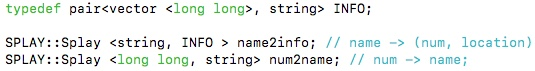
\includegraphics[width = 11cm]{def.jpeg}
			\end{center}
\section{附录}
	\subsection{程序中使用的一些宏}
			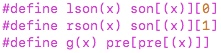
\includegraphics[width = 5cm]{define.jpeg}
		
\end{document}
